\chapter{Сложение скоростей, световые конусы и четырёхвекторы}

\section{Две системы отсчёта на одном железнодорожном пути}

Выведенное ранее преобразование Лоренца относилось к специально ограниченной геометрии: всё относительное движение происходило вдоль одной оси. Представим длинный железнодорожный путь. Один набор наблюдателей остаётся на станции; другой едет в поезде, движущемся вдоль пути. Поперечные направления существуют, но не играют роли, пока мы не восстановим их позднее.

Каждая система отсчёта представляет собой операционально определённую систему координат. Пространственные координаты задаются метровыми стержнями, покоящимися в этой системе, а время — синхронизированными часами, покоящимися в ней. Постулат, фиксирующий их связь, состоит в том, что каждый инерциальный наблюдатель измеряет одну и ту же скорость света.

В большинстве вычислений будет использоваться \(c=1\). Время можно измерять в секундах, а расстояние — в световых секундах, или в годах и световых годах. Тогда скорости становятся безразмерными долями скорости света. Когда нужны обычные единицы, множители \(c\) однозначно восстанавливаются из соображений размерности; например, \(v^2\) в безразмерном факторе Лоренца превращается в \(v^2/c^2\).

\subsection{Прямое и обратное преобразования}

Пусть где-то в поезде или рядом с ним происходит вспышка. Это одно событие, независимо от того, кто его описывает. Наблюдатель на станции приписывает ему координаты \((x,t)\), а наблюдатель в поезде — \((x',t')\). В единицах \(c=1\),
\begin{align}
x'&=\gamma_v(x-vt),&
t'&=\gamma_v(t-vx),
\label{eq:sr2-direct}\\
\gamma_v&=\frac{1}{\sqrt{1-v^2}}.
\end{align}
Ньютон узнал бы смещение \(x-vt\); релятивистские изменения — это множитель \(\gamma_v\) и то, что \(x\) входит в \(t'\).

\begin{figure}[htbp]
\centering
\includegraphics[width=0.90\textwidth]{lecture_02_figure_01.png}
\caption{Прямое преобразование Лоренца, связывающее координаты станции \((x,t)\) с координатами поезда \((x',t')\).}
\lectureframe{00:07:52}
\end{figure}

Из принципа взаимности обратное преобразование получается заменой знака относительной скорости:
\begin{align}
x&=\gamma_v(x'+vt'),&
t&=\gamma_v(t'+vx').
\label{eq:sr2-inverse}
\end{align}
Станция не находится в абсолютном покое. Это всего лишь система, которую мы обозначили без штрихов, и поезд видит, что она движется со скоростью \(-v\).

\begin{figure}[htbp]
\centering
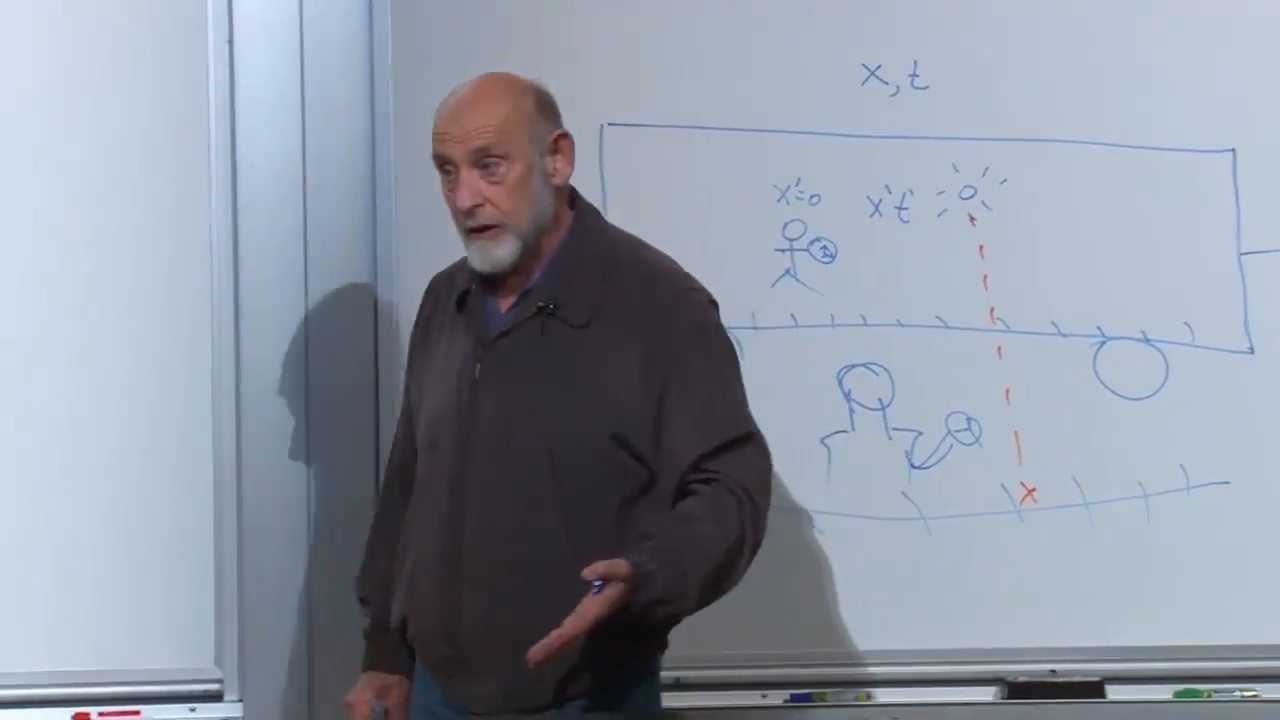
\includegraphics[width=0.90\textwidth]{lecture_02_figure_02.png}
\caption{Обратное преобразование имеет тот же фактор Лоренца и противоположный знак относительной скорости.}
\lectureframe{00:09:15}
\end{figure}

При бусте вдоль \(x\) поперечные координаты не изменяются:
\begin{equation}
y'=y,
\qquad
z'=z.
\end{equation}

Относительную скорость можно прочитать из пространственного уравнения, не анализируя его знаменатель. Начало координат поезда определяется условием \(x'=0\), и поэтому
\begin{equation}
x'=0
\quad\Longleftrightarrow\quad
x-vt=0
\quad\Longleftrightarrow\quad
x=vt.
\label{eq:sr2-origin-worldline}
\end{equation}
Коэффициент при \(t\) в этой мировой линии есть скорость поезда в координатах станции.

\section{Три системы отсчёта и композиция бустов}

Поместим внутрь поезда маленькую детскую тележку. Поезд движется со скоростью \(v\) относительно станции, а тележка катится по проходу со скоростью \(u\) относительно пассажира поезда. Скорость тележки относительно станции обозначим через \(w\). Ньютоновская интуиция подсказывает \(w=u+v\), но решать должны преобразования Лоренца.

Теперь имеются три системы координат:
\begin{equation}
(x,t),\qquad (x',t'),\qquad (x'',t'').
\end{equation}
Первая принадлежит станции, вторая — поезду, а третья — тележке. Между поездом и тележкой имеем
\begin{align}
x''&=\gamma_u(x'-ut'),&
t''&=\gamma_u(t'-ux'),
\label{eq:sr2-second-boost}\\
\gamma_u&=\frac{1}{\sqrt{1-u^2}}.
\end{align}

\begin{figure}[htbp]
\centering
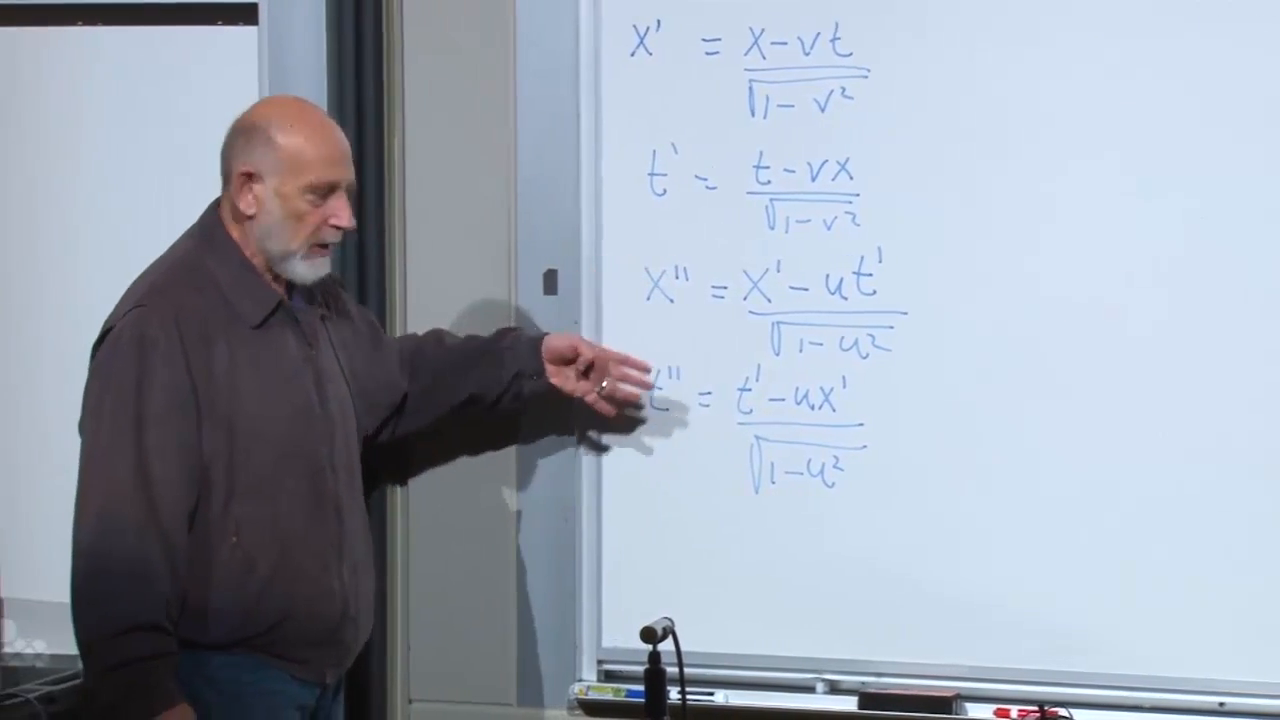
\includegraphics[width=0.90\textwidth]{lecture_02_figure_03.png}
\caption{За прямыми формулами перехода от станции к поезду следует второе преобразование Лоренца от штрихованных координат к дважды штрихованным.}
\lectureframe{00:14:55}
\end{figure}

\subsection{Подстановка одного буста в другой}

Пространственного уравнения достаточно, чтобы найти \(w\). Подставим \eqref{eq:sr2-direct} в первое уравнение из \eqref{eq:sr2-second-boost}:
\begin{align}
x''
&=\gamma_u(x'-ut')\\
&=\gamma_u\gamma_v\left[(x-vt)-u(t-vx)\right]\\
&=\gamma_u\gamma_v\left[(1+uv)x-(u+v)t\right].
\label{eq:sr2-composed-space}
\end{align}
Два знака минус в члене \(uvx\) дают плюс; два временных члена объединяются в \(-(u+v)t\).

\begin{figure}[htbp]
\centering
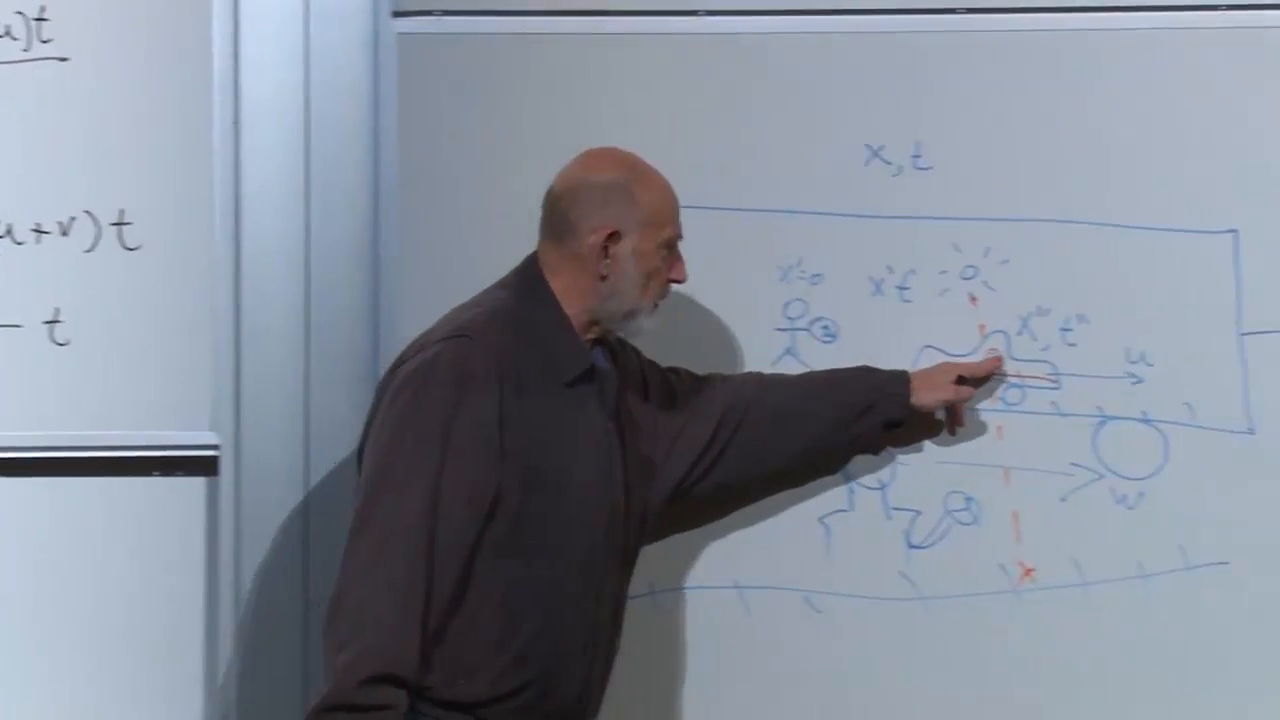
\includegraphics[width=0.91\textwidth]{lecture_02_figure_04.png}
\caption{Последовательная подстановка перед приведением членов с \(x\) и \(t\) в составном бусте.}
\lectureframe{00:16:30}
\end{figure}

Как и прежде, при нахождении движущегося начала координат знаменатель несуществен. Тележка покоится при \(x''=0\), поэтому скобка в \eqref{eq:sr2-composed-space} должна обращаться в нуль:
\begin{equation}
(1+uv)x-(u+v)t=0.
\end{equation}
Следовательно, её мировая линия в системе станции равна
\begin{equation}
x=\frac{u+v}{1+uv}\,t,
\end{equation}
а её скорость равна
\begin{equation}
\boxed{w=\frac{u+v}{1+uv}}.
\label{eq:sr2-velocity-add-c1}
\end{equation}

\begin{figure}[htbp]
\centering
\includegraphics[width=0.91\textwidth]{lecture_02_figure_05.png}
\caption{Собранный числитель и мировая линия \(x=[(u+v)/(1+uv)]t\) дают составную скорость.}
\lectureframe{00:19:30}
\end{figure}

Временное уравнение при композиции тоже ведёт себя согласованно. Полное преобразование от станции к тележке имеет лоренцеву форму
\begin{align}
x''&=\gamma_w(x-wt),&
t''&=\gamma_w(t-wx),
\end{align}
где
\begin{equation}
\gamma_w=\frac{1}{\sqrt{1-w^2}}.
\end{equation}
Действительно,
\begin{equation}
\gamma_w=\gamma_u\gamma_v(1+uv),
\end{equation}
что получается подстановкой \eqref{eq:sr2-velocity-add-c1} и упрощением. Следовательно, два коллинеарных буста дают ещё один коллинеарный буст.

\subsection{Восстановление размерностей}

\begin{classroomqa}
\audiencequestion{Почему знаменатель \(1+uv\) размерно некорректен в обычных единицах?}
\lecturerresponse{Он правилен только потому, что \(c=1\) делает каждую скорость безразмерной долей скорости света. В обычных единицах это произведение должно иметь вид \(uv/c^2\), и тогда оно безразмерно. \lecturetimestamp{00:21:11}}
\end{classroomqa}

Размерный закон сложения скоростей имеет вид
\begin{equation}
\boxed{
w=\frac{u+v}{1+\dfrac{uv}{c^2}}
}.
\label{eq:sr2-velocity-add}
\end{equation}

\begin{figure}[htbp]
\centering
\includegraphics[width=0.90\textwidth]{lecture_02_figure_06.png}
\caption{Требование размерной согласованности возвращает \(c^2\) под произведением \(uv\).}
\lectureframe{00:22:06}
\end{figure}

При \(\lvert u\rvert,\lvert v\rvert\ll c\),
\begin{equation}
\frac{uv}{c^2}\ll 1,
\end{equation}
поэтому
\begin{equation}
w\approx u+v.
\end{equation}
Ньютоновское сложение — это низкоскоростное приближение, а не отдельное правило.

\subsection{Два численных режима}

Сначала возьмём
\begin{equation}
u=v=0.01c.
\end{equation}
В единицах \(c=1\),
\begin{equation}
w=\frac{0.02}{1.0001}\approx 0.019998.
\end{equation}
1 процент скорости света — это уже примерно \(3\times10^6\ {\rm m/s}\), однако релятивистская поправка составляет лишь одну десятитысячную. Результат немного меньше ньютоновского \(0.02c\).

\begin{figure}[htbp]
\centering
\includegraphics[width=0.90\textwidth]{lecture_02_figure_07.png}
\caption{При \(u=v=0.01c\) знаменатель отличается от единицы лишь на \(10^{-4}\).}
\lectureframe{00:24:23}
\end{figure}

Теперь возьмём
\begin{equation}
u=v=0.9c.
\end{equation}
Ньютон предсказал бы \(1.8c\). Теория относительности даёт
\begin{equation}
\frac{w}{c}
=\frac{0.9+0.9}{1+0.9^2}
=\frac{1.8}{1.81}
\approx 0.9945.
\label{eq:sr2-fast-example}
\end{equation}

\begin{figure}[htbp]
\centering
\includegraphics[width=0.90\textwidth]{lecture_02_figure_08.png}
\caption{Две скорости \(0.9c\) дают \(1.8/1.81\), что всё ещё меньше скорости света.}
\lectureframe{00:25:48}
\end{figure}

Последовательные досветовые бусты не могут перейти через \(c\). Если \(u<c\) и \(v<c\), то
\begin{equation}
1-\frac{w}{c}
=
\frac{\left(1-\frac{u}{c}\right)
      \left(1-\frac{v}{c}\right)}
     {1+\frac{uv}{c^2}}
>0.
\end{equation}
Каждый дополнительный буст может приблизить результат к \(c\), но никогда не переведёт его за эту границу. При предельном значении \(u=c\),
\begin{equation}
w=\frac{c+v}{1+v/c}=c.
\end{equation}
Скорость света является неподвижной точкой закона композиции.

\section{Координатное измерение — не визуальная картина}

\begin{classroomqa}
\audiencequestion{Если у поезда стеклянные стены, может ли наблюдатель на станции просто посмотреть на пассажира и тележку вместе и непосредственно определить их движения?}
\lecturerresponse{Преобразование Лоренца относится к координатным измерениям, выполняемым с помощью разнесённых в пространстве линеек и синхронизированных часов. Зрительный образ тоже включает неодинаковые времена прохождения света от разных событий к наблюдателю. Стекло меняет вид, но не координатную связь, а принятие одного изображения за одновременные данные вновь ввело бы то самое предположение об одновременности, которое исправила теория относительности. \lecturetimestamp{00:27:53}}
\end{classroomqa}

Событие имеет место и время в каждой системе отсчёта независимо от того, увидит ли его кто-нибудь в этот момент или нет. Оптический облик — вполне законный предмет рассмотрения, но он требует второго расчёта, в котором прослеживается свет от каждого события до глаза. Сами законы преобразования универсальны и не зависят от стен поезда.

\section{Собственный интервал в трёх пространственных измерениях}

Вернёмся к двум событиям: одно из них находится в начале координат, а другое — в \((x,t)\). В одном пространственном измерении,
\begin{equation}
\tau^2=t^2-x^2
\label{eq:sr2-interval-1d}
\end{equation}
в единицах \(c=1\). Все инерциальные системы отсчёта согласны с тем, что
\begin{equation}
\tau^2
=t^2-x^2
=t'^2-x'^2
=t''^2-x''^2.
\end{equation}
Координаты меняются; собственный интервал — нет.

При времениподобном разделении часы могут переместиться между этими событиями. Если в первом событии они показывают полдень, то прошедшее по ним время ко второму событию есть собственное время \(\tau\). Это утверждение не зависит от того, в какой системе координат вычисляется интервал.

\begin{figure}[htbp]
\centering
\includegraphics[width=0.90\textwidth]{lecture_02_figure_09.png}
\caption{Перед восстановлением поперечных направлений напомним инвариантное соотношение для собственного времени \(\tau^2=t^2-x^2\).}
\lectureframe{00:30:18}
\end{figure}

\subsection{Пространственные повороты восстанавливают поперечные направления}

Прежде чем вернуться к бустам, рассмотрим обычный поворот пространственных осей. Для точки, не лежащей на оси \(x\), квадрат пространственного расстояния равен
\begin{equation}
r^2=x^2+y^2+z^2,
\end{equation}
и по обычной теореме Пифагора инвариантен относительно поворотов. Следовательно, интервал в \(3+1\)-мерном пространстве-времени равен
\begin{equation}
\boxed{
\tau^2=t^2-x^2-y^2-z^2
}.
\label{eq:sr2-interval-3d}
\end{equation}
После восстановления \(c\) получаем
\begin{equation}
c^2\tau^2
=c^2t^2-x^2-y^2-z^2.
\end{equation}

\begin{figure}[htbp]
\centering
\includegraphics[width=0.90\textwidth]{lecture_02_figure_10.png}
\caption{Пифагорово пространственное расстояние расширяет инвариант \(t^2-x^2\) до \(t^2-x^2-y^2-z^2\).}
\lectureframe{00:34:23}
\end{figure}

Любая комбинация пространственных поворотов и лоренцевых бустов сохраняет \eqref{eq:sr2-interval-3d}. Обычные координатные оси дают разные компоненты, но одно и то же евклидово расстояние; инерциальные системы отсчёта дают разные пространственные и временные компоненты, но одну и ту же эту разность квадратов. Этот инвариант — центральный геометрический факт специальной теории относительности.

\begin{classroomqa}
\audiencequestion{Если пассажир заменит игрушечную машинку направленным вперёд лучом фонарика, получат ли наблюдатели в поезде и на станции одну и ту же скорость света?}
\lecturerresponse{Подставим \(u=c\) в \eqref{eq:sr2-velocity-add}. Тогда \(w=(c+v)/(1+v/c)=c\). В единицах \(c=1\) это отношение просто равно \((1+v)/(1+v)=1\). Обе системы отсчёта измеряют одну и ту же скорость, в точности как и требуется. \lecturetimestamp{00:35:53}}
\end{classroomqa}

Следовательно, прежнее затруднение со стеклянной стеной не означает нарушения инвариантности скорости света. Это путаница между координатным измерением и изображением, увиденным с запаздыванием, а в конечном счёте — путаница относительно одновременности.

\section{Нулевые лучи и световой конус}

В одном пространственном измерении световые лучи, идущие вправо и влево, удовлетворяют
\begin{equation}
x=\pm t.
\end{equation}
Их интервал обращается в нуль:
\begin{equation}
t^2-x^2=0.
\end{equation}
В отличие от евклидова расстояния, нулевой пространственно-временной интервал не требует совпадения событий. Он означает, что их может соединить световой сигнал.

После восстановления всех пространственных направлений световой луч удовлетворяет
\begin{equation}
t^2-x^2-y^2-z^2=0,
\label{eq:sr2-null}
\end{equation}
или
\begin{equation}
r=t
\end{equation}
для света, направленного в будущее, в единицах \(c=1\).

\begin{figure}[htbp]
\centering
\includegraphics[width=0.90\textwidth]{lecture_02_figure_11.png}
\caption{Свет в любом пространственном направлении следует нулевой траектории, удовлетворяющей \(t^2-(x^2+y^2+z^2)=0\).}
\lectureframe{00:39:28}
\end{figure}

В \(1+1\) измерениях нулевое множество представляет собой пару прямых под углом \(45^\circ\). При двух пространственных измерениях и времени оно становится конусом; три пространственных измерения нельзя полностью изобразить на доске, но определяющее уравнение остаётся тем же.

Будущий световой конус состоит из событий, которых может достичь свет, испущенный из начала координат. Прошлый световой конус состоит из событий, из которых свет может достичь начала координат. Один — это другой, перевёрнутый по времени.

\begin{figure}[htbp]
\centering
\includegraphics[width=0.90\textwidth]{lecture_02_figure_12.png}
\caption{Нулевые лучи под углом \(45^\circ\) образуют будущий и прошлый световые конусы на рисунке пространства-времени большей размерности.}
\lectureframe{00:40:47}
\end{figure}

\begin{classroomqa}
\audiencequestion{Каков соответствующий инвариант при галилеевых преобразованиях в ньютоновской механике?}
\lecturerresponse{Сам временной интервал. Все наблюдатели в ньютоновской механике согласны относительно \(\Delta t\), хотя они расходятся в пространственном смещении. Теория относительности отказывается от универсального времени и заменяет его инвариантным пространственно-временным интервалом. \lecturetimestamp{00:41:53}}
\end{classroomqa}

\section{От пространственных векторов к четырёхвекторам}

Векторы здесь — это геометрические векторы, а не векторы квантовых состояний. Смещение между двумя точками в обычном пространстве имеет длину и направление. Его начало можно перенести в начало координат, не изменяя самого вектора, и его три компоненты можно обозначить как
\begin{equation}
x^i=(x^1,x^2,x^3)=(x,y,z),
\qquad i=1,2,3.
\end{equation}
Латинский индекс \(i\) пробегает только пространственные направления.

Для события нужна ещё одна компонента — его время. Поэтому положение в пространстве-времени записывается как
\begin{equation}
x^\mu=(x^0,x^1,x^2,x^3)=(t,x,y,z),
\qquad \mu=0,1,2,3.
\label{eq:sr2-four-position}
\end{equation}
По историческому соглашению время является нулевой компонентой, а не четвёртой:
\begin{equation}
x^0=t,\qquad x^1=x,\qquad x^2=y,\qquad x^3=z.
\end{equation}
Греческие индексы, такие как \(\mu\), пробегают пространство-время; латинские индексы, такие как \(i\), пробегают пространство.

\begin{figure}[htbp]
\centering
\includegraphics[width=0.90\textwidth]{lecture_02_figure_13.png}
\caption{Пространственные компоненты \(x^i\) расширяются до четырёхкомпонентного положения в пространстве-времени \(x^\mu=(x^0,x^1,x^2,x^3)\).}
\lectureframe{00:46:05}
\end{figure}

Инвариант принимает вид
\begin{equation}
\tau^2
=(x^0)^2-(x^1)^2-(x^2)^2-(x^3)^2.
\end{equation}
Само по себе это обозначение не добавляет никакой новой физики. Его ценность состоит в том, что преобразование Лоренца действует линейно на все четыре компоненты, точно так же как поворот действует линейно на пространственный вектор.

\begin{classroomqa}
\audiencequestion{Поскольку преобразование линейно, можно ли представить его матрицей, действующей на вектор-столбец?}
\lecturerresponse{Да. Для буста вдоль \(x\) нетривиальный блок \(\gamma_v\begin{pmatrix}1&-v\\-v&1\end{pmatrix}\) действует на \((t,x)^{\mathsf T}\), тогда как \(y\) и \(z\) не изменяются. Матричная запись — естественный способ составлять и упорядочивать преобразования Лоренца. \lecturetimestamp{00:48:14}}
\end{classroomqa}

Явно,
\begin{equation}
\begin{pmatrix}
t'\\x'\\y'\\z'
\end{pmatrix}
=
\begin{pmatrix}
\gamma_v&-\gamma_v v&0&0\\
-\gamma_v v&\gamma_v&0&0\\
0&0&1&0\\
0&0&0&1
\end{pmatrix}
\begin{pmatrix}
t\\x\\y\\z
\end{pmatrix}.
\label{eq:sr2-boost-matrix}
\end{equation}

\section{Смещения и четырёхскорость}

Теперь перейдём от положения одного события к короткому участку мировой линии частицы. Четырёхсмещение равно
\begin{equation}
\Delta x^\mu
=(\Delta t,\Delta x,\Delta y,\Delta z).
\end{equation}
Когда смещение называют малым, это значит, что мы приближаемся к исчислению: \(\Delta x^\mu\) станет \(dx^\mu\). Пока что конечная запись делает геометрию наглядной.

Приращение собственного времени вдоль времениподобной мировой линии удовлетворяет соотношению
\begin{equation}
(\Delta\tau)^2
=(\Delta t)^2-(\Delta x)^2-(\Delta y)^2-(\Delta z)^2.
\label{eq:sr2-proper-increment}
\end{equation}
Обычная скорость есть пространственное смещение, делённое на координатное время, и имеет три компоненты. Четырёхскорость же есть четырёхсмещение, делённое на инвариантное собственное время:
\begin{equation}
u^\mu
=\frac{\Delta x^\mu}{\Delta\tau}
\quad\longrightarrow\quad
\boxed{
u^\mu=\frac{dx^\mu}{d\tau}
}.
\label{eq:sr2-four-velocity}
\end{equation}

\begin{figure}[htbp]
\centering
\includegraphics[width=0.90\textwidth]{lecture_02_figure_14.png}
\caption{Участок мировой линии задаёт \(\Delta x^\mu\), его инвариант \(\Delta\tau\) и четырёхскорость \(u^\mu=\Delta x^\mu/\Delta\tau\).}
\lectureframe{00:52:42}
\end{figure}

Этот объект имеет четыре компоненты и преобразуется как четырёхвектор. Его связь с обычной трёхскоростью — следующий вопрос, который здесь намеренно оставлен открытым. Его разрешение ведёт к релятивистскому импульсу, релятивистской энергии, релятивистскому ускорению и, в конечном счёте, к релятивистскому обобщению \(F=ma\).
